\section{Лабораторная работа 3 (вариант 5-8)}

\subsection{Задание}
Цель работы - создание программы, реализующей искусственный нейрон; разработка процедуры обучения нейрона; использование полученных результатов для решения тестовых задач классификации и аппроксимации.

\subsection{WTA нейрон}
Нейроны типа WTA (Winner Takes All — победитель получает все) всегда используются группами, в которых конкурируют между собой. Структурная схема группы (слоя) нейронов типа WTA представлена на рисунке ниже (рисунок \ref{img:wta}).

\begin{figure}[H]
\centering
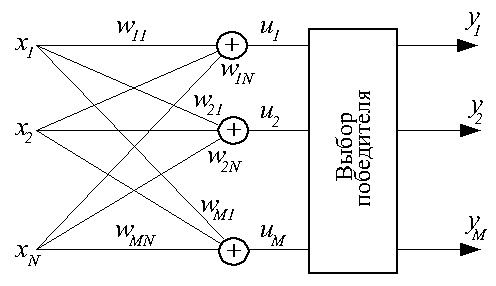
\includegraphics[scale=0.5]{wta.png}
\caption{Структурная схема слоя нейрона типа WTA}
\label{img:wta}
\end{figure}

Каждый конкурирующий нейрон в группе получает одни и те же входные сигналы. Каждый нейрон рассчитывает выходной сигнал своего сумматора обычным образом:

\begin{equation}\label{eq:minFunc}
	u_i=\sum\limits_{j=0}^N w_{ij}*x_j.
\end{equation}

\begin{itemize}
\item По результатам сравнения всех $u_i, j=1, 2, ..., M$ выбирается нейрон-победитель, обладающий наибольшим значением $u_i$. Выходной сигнал $y_i$ нейрона-победителя получает значение 1, выходные сигналы всех остальных нейронов — 0.
\end{itemize}

Для обучения нейронов типа WTA не требуется учитель, оно практически полностью аналогично обучению инстара Гроссберга. Начальные значения весовых коэффициентов всех нейронов выбираются случайным образом с последующей нормализацией относительно 1.
При предъявлении каждого обучающего вектора $X^k$ определяется нейрон-победитель, что дает ему право уточнить свои весовые коэффициенты по упрощенному (в силу бинарности $y_i$) правилу Гроссберга:

\begin{equation}\label{eq:minFunc}
    w_{ij}(t+1)=w_{ij}(t)+\eta(x_j^k-w_{ij}(t)).
\end{equation}
Все проигравшие нейроны оставляют свои весовые коэффициенты неизменными. 

В каждом цикле обучения побеждает тот нейрон, чей текущий вектор входных весов $W_i$ наиболее близок входному вектору $X_k$. При этом вектор $W_i$ корректируется в сторону вектора $X_k$. Поэтому в ходе обучения каждая группа близких друг другу входных векторов (кластер) обслуживается отдельным нейроном.


















--------------------------------------------------------------------------------------------------------------------------------


Выходной сигнал нейрона может принимать только два значения {0, 1} по следующему правилу:

\begin{equation}\label{eq:system}
		\begin{aligned}
  			& y_i = f(u_i)=1, если u_i>=0, \\
  			& y_i = f(u_i)=0, если u_i<0.
		\end{aligned}  		
\end{equation}


Обучение персептрона требует учителя, т.е. множества ${<X^1, d^1_i>, ..., <X^p, d^p_i>}$ пар $<вектор входных сигналов X^k, ожидаемое значение выходного сигнала d^k_i>$. Обучение (отыскание весовых коэффициентов $w_{ij}$) сводится к задаче минимизации целевой функции:

\begin{equation}\label{eq:minFunc}
	E(W_i)=\dfrac{1}{2}\sum\limits_{k=1}^p(y^k_i-d^k_i)^2.
\end{equation}

К сожалению, для персептрона в силу разрывности функции $f(u_i)$ для отыскания минимума $E(W_i)$ применимы методы оптимизации только нулевого порядка.

На практике для обучения персептрона чаще всего используется правило персептрона, представляющее собой следующий простой алгоритм:

\begin{itemize}
\item Выбираются (как правило, случайно) начальные значения весов $w_{ij} (j=0, 1, 2, ..., N)$ нейрона.

\item Для каждой обучающей пары $<X^k, d^k_i>$ выполняется ряд циклов (их номера обозначим через $t$) уточнения значений входных весов по формуле
\begin{equation}
  w_{ij}(t+1) = w_{ij}(t) + \Delta w_{ij}(t),
\end{equation}
где
\begin{equation}\label{eq:system}
	\begin{aligned}
	& \Delta w_{ij}(t)=0, если y_i(t)=d^k_i; \\
	& \Delta w_{ij}(t)=x^k_j, если y_i(t)=0, а d^k_i=1; \\
	& \Delta w_{ij}(t)=-x^k_j, если y_i(t)=1, а d^k_i=0. 
	\end{aligned}  		
\end{equation}

\item Процесс обработки текущей обучающей пары завершается:
	\begin{enumerate}
	\item[] либо а) на цикле, в котором все $\Delta w_{ij}(t)=0$ ,
	\item[] либо б) после достижения предельного количества циклов.
	\end{enumerate}
\end{itemize}

Следует отметить, что правило персептрона представляет собой частный случай предложенного много позже универсального правила обучения Видроу-Хоффа:
\begin{equation}\label{eq:vidHoff}
  \Delta w_{ij}(t)=x^k_j(d^k_i-y_i(t)).
\end{equation}

\subsection{Исходные данные}

Обучающие данные для варианта 6 представлены на рисунке \ref{img:data_lab2}.

\begin{figure}[H]
\centering
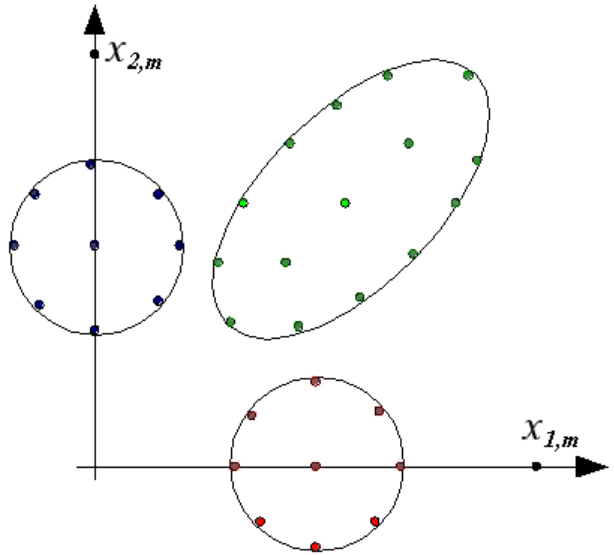
\includegraphics[scale=0.5]{data_lab2.png}
\caption{Данные для обучения варианта 6}
\label{img:data_lab2}
\end{figure}

\subsection{Обучение}

Среди точек на рисунке \ref{img:data_lab2} выбраны те, которые принадлежат синей и зеленой областям. Обучение происходит только на этих двух множествах.

Сгенерированные программно обучающие данные выглядят следующим образом:

\begin{figure}[H]
\centering
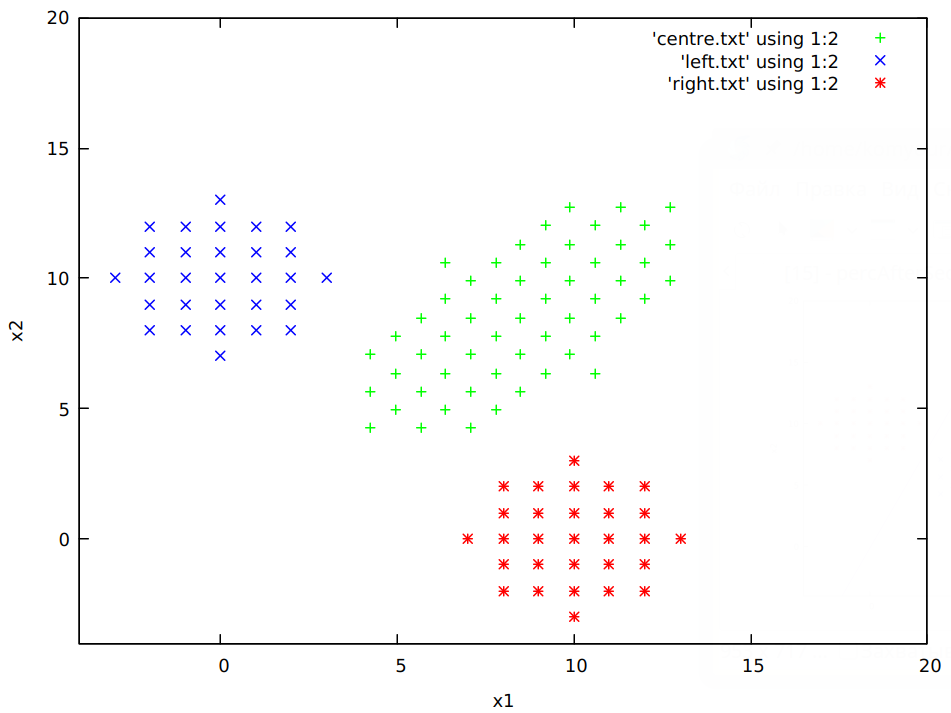
\includegraphics[scale=0.5]{percPrepData.png}
\caption{Обучающие данные}
\label{img:}
\end{figure}

Начальные веса принимаются равными 0.1.

Обучение ведется онлайн-методом, то есть минимизация целевой функции \eqref{eq:minFunc} выполняется для каждого входного вектора.

Подстройка весов выполняется по правилу Видроу-Хоффа \eqref{eq:vidHoff}.

В цикле настройки весов ограничение стоит не только на величину ошибки (которая на текущем шаге должна стать равной 0), но и на количество итераций (задано как 100, хотя на деле больше 2-3 не требуется).

Для хорошей классификации выбранных данных достаточно выполнить два прохода по набору обучающих данных, то есть две эпохи.

После первой эпохи классификация выполняется с ошибкой:

\begin{figure}[H]
\centering
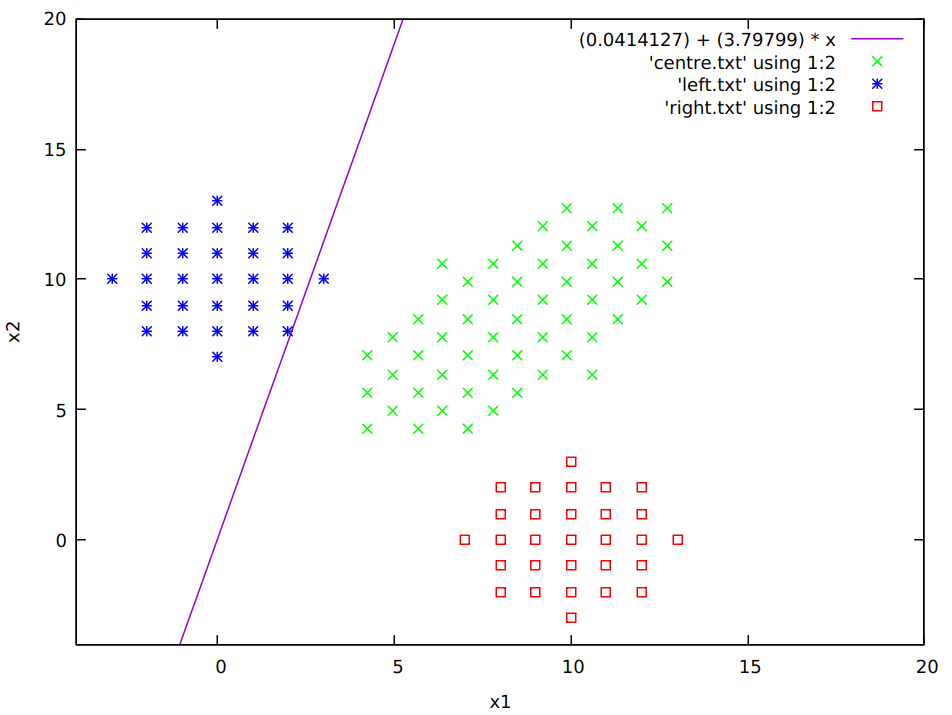
\includegraphics[scale=0.5]{percAfterFirstEpoch.png}
\caption{Классификация после первой эпохи}
\label{img:}
\end{figure}

Результат обучения:

\begin{figure}[H]
\centering
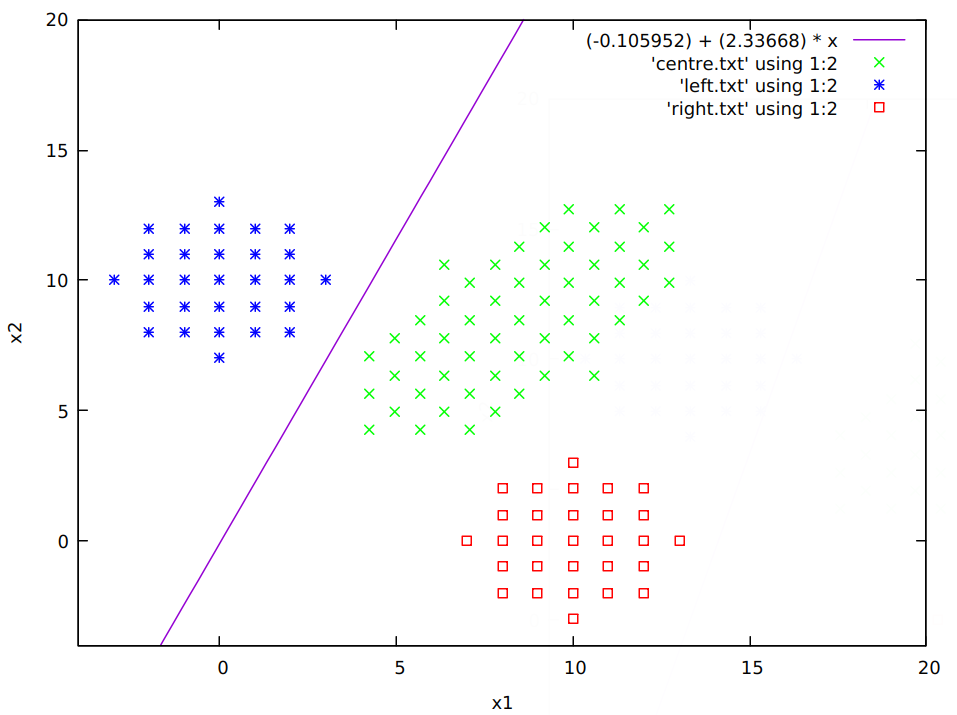
\includegraphics[scale=0.5]{percAfterSecondEpoch.png}
\caption{Классификация после второй эпохи}
\label{img:}
\end{figure}

\subsection{Иходный код}
Файл main.cpp
\begin{verbatim}
     1  #include <cmath>
     2  #include <vector>
     3  #include <fstream>
     4  #include <iostream>
     5  #include <algorithm>
     6
     7  #include "Perceptron.h"
     8
     9  // -----------------------------------------------------------
-----------------
    10  void prepareOutputFile(std::ofstream &file)
    11  {
    12      file << "set xrange[" << -4 << ":" << 20 << "]" << std::en
dl;
    13      file << "set yrange[" << -4 << ":" << 20 << "]" << std::en
dl;
    14      file << "set xlabel 'x1'" << std::endl;
    15      file << "set ylabel 'x2'" << std::endl;
    16  }
    17  // -----------------------------------------------------------
-----------------
    18  std::vector<DataSample>& concat(std::vector<DataSample> &a, st
d::vector<DataSample> &b)
    19  {
    20      a.insert(a.end(), b.begin(), b.end());
    21      return a;
    22  }
    23  // -----------------------------------------------------------
-----------------
    24  void generateEllipsoid(double a, double b, 
    25                         double x0, double y0, 
    26                         double angle, double step, 
    27                         int group,
    28                         std::vector<DataSample> &dataset,
    29                         std::ofstream &file)
    30  {
    31      angle = -angle; 
    32      for( double x = x0 - a; x <= x0 + a; x += step){
    33          for(double y = y0 - b; y <= y0 + b; y += step){
    34              if(pow(x - x0, 2)/pow(a, 2) + pow(y - y0, 2)/pow(b
, 2) <= 1){
    35                  double xEllispe = (x)*cos(angle) + (y)*sin(ang
le);
    36                  double yEllispe = -(x)*sin(angle) + (y)*cos(an
gle);
    37                  DataSample set = {{xEllispe, yEllispe}, group}
;
    38                  dataset.push_back(set);
    39                  file << xEllispe << "\t" << yEllispe << std::e
ndl;
    40              }
    41          }
    42      }
    43      return ;
    44  }
    45  // -----------------------------------------------------------
-----------------
    46  int main()
    47  {
    48      std::ofstream left("left.txt");
    49      std::ofstream centre("centre.txt");
    50      std::ofstream right("right.txt");
    51
    52      std::vector<DataSample> setA, setB, setC;
    53      generateEllipsoid(3, 3, 10, 0, 0, 1., 0, setA, right);
    54      generateEllipsoid(3, 3, 0, 10, 0, 1, 0, setB, left);
    55      generateEllipsoid(6, 3, 12, 0, atan(1.), 1., 1, setC, cent
re);
    56
    57      std::vector<DataSample> dataset = concat(setB, setC);
    58
    59      std::ofstream file("output.txt");
    60      prepareOutputFile(file);
    61
    62      Perceptron neuron(dataset);
    63      neuron.train(file);
    64
    65      return 0;
    66  }
\end{verbatim}

Файл Perceptron.h
\begin{verbatim}
     1  #ifndef NEURON_PERCEPTRON_H
     2  #define NEURON_PERCEPTRON_H
     3
     4  #include <vector>
     5  #include <fstream>
     6
     7
     8  struct DataSample {
     9      std::vector<double> X;
    10      int y;
    11  };
    12
    13  class Perceptron {
    14  protected:
    15      std::vector<double>         m_weights;
    16      std::vector<DataSample> m_dataset;
    17  public:
    18          Perceptron() {};
    19      Perceptron(std::vector<DataSample> &dataset): m_dataset(da
taset) {};
    20      ~Perceptron() {};
    21      void train(std::ofstream &file);
    22          void updateOutputFile(std::ofstream &file, std::vector
<double> &weights);
    23  };
    24
    25  int heaviside(double x);
    26  #endif
\end{verbatim}

Файл Perceptron.cpp
\begin{verbatim}
     1  #include <cmath>
     2  #include <fstream>
     3  #include <iostream>
     4  #include <algorithm>
     5
     6  #include "Perceptron.h"
     7
     8  void Perceptron::train(std::ofstream &file) {
     9      unsigned int epoch;
    10      m_weights = std::vector<double>(m_dataset.front().X.size()
 + 1, 0.1);
    11      updateOutputFile(file, m_weights);
    12      for (epoch = 0; epoch < 2; epoch++) {
    13          std::random_shuffle(m_dataset.begin(), m_dataset.end()
);
    14          for (auto set : m_dataset) {
    15              std::vector<double> X = set.X;
    16              X.insert(X.begin(), 1.);
    17              bool errors = true; 
    18              for (int iterCounter = 0; iterCounter < 100 && err
ors; iterCounter++) {  
    19                  errors = false;
    20                  double weightedSum = 0.; //m_weights * X; 
    21                  for (int i = 0; i < m_weights.size(); i++) {
    22                          weightedSum += m_weights[i] * X[i];
    23                  }          
    24                  double y = heaviside(weightedSum);
    25                  for (auto itX : (X)) {
    26                      if (itX*(set.y - y)) {
    27                          errors = true;
    28                      }
    29                  }
    30                  if (errors) {
    31                      for (int i = 0; i < m_weights.size(); i++)
 {
    32                          m_weights[i] = m_weights[i] + X[i]*(se
t.y - y);
    33                      }            
    34                      updateOutputFile(file, m_weights);
    35                  }
    36              }
    37              updateOutputFile(file, m_weights);
    38          }
    39      }
    40  }
    41  // -----------------------------------------------------------
-----------------
    42  void Perceptron::updateOutputFile(std::ofstream &file, std::ve
ctor<double> &weights)
    43  {
    44      file << "plot (" << -weights[0] / weights[2] << ") + (" <<
 -weights[1] / weights[2] << ") * x, \\" << std::endl;
    45      file << "'centre.txt' using 1:2 w p lt rgb 'green', \\" <<
 std::endl;
    46      file << "'left.txt' using 1:2 w p lt rgb 'blue', \\" << st
d::endl;
    47      file << "'right.txt' using 1:2 w p lt rgb 'red'" << std::e
ndl;
    48      file << "pause 0.1" << std::endl;
    49  }
    50  // -----------------------------------------------------------
-----------------
    51  int heaviside(double x) {
    52      return x < 0 ? 0 : 1;
    53  }
    54
\end{verbatim}
